\documentclass[10.5pt,scale=1.0,t,aspectratio=169,hyperref={pdfpagelabels=false}]{beamer}
%\usepackage[paperwidth=13.33in, paperheight=7.5in,top=.25in, bottom=.25in, left=.25in, right=.25in]{geometry}
%\geometry{papersize={13.33in,7.5in}}

%\usetheme{Dresden}
%\usetheme{Warsaw}

%Other themes
%https://hartwork.org/beamer-theme-matrix/

\usepackage{lipsum}
\usepackage{color}

\usepackage{amsfonts}
\usepackage{amsmath,mathtools}
\usepackage{mathrsfs}
\usepackage{array}
\usepackage{algorithm}
\usepackage{hyperref}
\usepackage[spanish,es-nodecimaldot]{babel}
\usepackage[utf8]{inputenc}
%\usepackage{intcalc}
\usepackage{graphicx}
\usepackage{multicol}
%\usepackage{authblk}
\usepackage{multirow}
\usepackage{enumitem}
\usepackage[document]{ragged2e}

\usepackage[absolute,overlay]{textpos}
\textblockorigin{0mm}{0mm} 

\usefonttheme[onlymath]{serif}
%\usepackage{epstopdf}
\usepackage{verbatim}
\usepackage{cite}
%\usepackage[texcoord,grid,gridunit=mm,gridcolor=red!10,subgridcolor=green!10]{eso-pic}




\newenvironment{conditions}[1][where:]
{#1 \begin{tabular}[t]{>{$}l<{$} @{${}={}$} l}}
	{\end{tabular}\\[\belowdisplayskip]}


\newcolumntype{L}{>{$}l<{$}} % math-mode version of "l" column type


\newcounter{saveenumi}
\newcommand{\seti}{\setcounter{saveenumi}{\value{enumi}}}
\newcommand{\conti}{\setcounter{enumi}{\value{saveenumi}}}

\setbeamertemplate{bibliography item}{\insertbiblabel}


\hypersetup{colorlinks=true,
	linkcolor=blue,
	linktoc=all,				
	citecolor=blue,
	urlcolor=red,
	pdftitle={FUNDAMENTOS DE AUTOMATIZACIÓN Y CONTROL},
	pdfauthor={Santiago Rúa Pérez},
	pdfcreator={Santiago Rúa Pérez}}


\definecolor{GreenDark}{rgb}{0.0, 0.60, 0.0}
\definecolor{RedDark}{rgb}{183, 0.0, 0.0}
\definecolor{BlueDark}{rgb}{0.0, 0.0, 167}
\definecolor{BlueLight}{rgb}{0.2, 0.451, 0.517}


\graphicspath{{imag/}}

\newcommand{\Ho}{$H_{0}$}
\newcommand{\Ha}{$H_{a}$}
\newcommand{\Nota}{{\bf Nota: }}
\newcolumntype{P}[1]{>{\centering\arraybackslash}p{#1}}
\newcolumntype{M}[1]{>{\centering\arraybackslash}m{#1}}

\newcommand{\less}{<}
\newcommand{\greater}{>}


\setlength{\parindent}{1em}
\setlength{\parskip}{.6em}
\renewcommand{\baselinestretch}{.9}

%%%%    C environment    ---------------- %%%%%%%%%%%%%%%.
\usepackage{listings}
\usepackage{xcolor}
\definecolor{mGreen}{rgb}{0,0.6,0}
\definecolor{mGray}{rgb}{0.5,0.5,0.5}
\definecolor{mPurple}{rgb}{0.58,0,0.82}
\definecolor{backgroundColour}{rgb}{0.95,0.95,0.92}

\lstdefinestyle{CStyle}{
	backgroundcolor=\color{backgroundColour},   
	commentstyle=\color{mGreen},
	keywordstyle=\color{magenta},
	numberstyle=\tiny\color{mGray},
	stringstyle=\color{mPurple},
	basicstyle=\tiny,
	breakatwhitespace=false,         
	breaklines=true,                 
	captionpos=b,                    
	keepspaces=true,                 
	numbers=left,                    
	numbersep=5pt,                  
	showspaces=false,                
	showstringspaces=false,
	showtabs=false,                  
	tabsize=2,
	language=C
}
%%--------------------------------------------------------------------------


\title{Electrónica Digital II}   
\author{Santiago Rúa Pérez, PhD.} 
\date{\today} 

\setlength{\TPHorizModule}{\textwidth}
\setlength{\TPVertModule}{\textwidth}

\newcommand{\btVFill}{\vskip0pt plus 1filll}


\setbeamertemplate{sidebar right}{}
\setbeamertemplate{footline}
{
	\leavevmode%
	\hbox{%
		\begin{beamercolorbox}[wd=.333333\paperwidth,ht=2.25ex,dp=1ex,center]{author in head/foot}%
			\usebeamerfont{author in head/foot}\insertshortauthor
		\end{beamercolorbox}%
		\begin{beamercolorbox}[wd=.333333\paperwidth,ht=2.25ex,dp=1ex,center]{title in head/foot}%
			\usebeamerfont{title in head/foot}\insertshorttitle
	\end{beamercolorbox}}%
	\vskip0pt%
}
\makeatother

\begin{document}
%%%%%%%%%%%%%%%%%% FRAME %%%%%%%%%%%%%%%%%%%%%%%%%%
\begin{frame}
	\titlepage
\end{frame}
%%%%%%%%%%%%%%%%% FRAME START %%%%%%%%%%%%%%%%%%%%%%%%%%
\frame{
%\frametitle{}
\begin{center}
\LARGE \textcolor{blue}{PROGRAMACIÓN ESTRUCTURADA EN C}
\end{center}
 
}
%%%%%%%%%%%%%%%%% FRAME START %%%%%%%%%%%%%%%%%%%%%%%%%%

%%%%%%%%%%%%%%%%% FRAME %%%%%%%%%%%%%%%%%%%%%%%%%%
\begin{frame}
	\frametitle{Programación estructurada en C}
	{\bf Objetivos}
	\begin{itemize}
	\item Entender los bucles por centinela y contador.
	\item Entender ciclos for.
	\item Entender ciclos do while.
	\item Comando break and continue.
	\item Operadores lógicos.
	\end{itemize}
\end{frame}
%%%%%%%%%%%%%%%%% FRAME %%%%%%%%%%%%%%%%%%%%%%%%%%
\begin{frame}[fragile]
	\frametitle{Iteracion controlada por contador}
	\begin{itemize}
		\item El nombre de una variable de control.
		\item Un valor inicial de esa variable de control.
		\item Un incremento o decremento de la señal de control.
		\item Una condicion de valor final. 
	\end{itemize}

	\begin{lstlisting}[style=CStyle]
		// Iteracion controlada por contador
		#include <stdio.h>
		
		int main(void)
		{
			unsigned int counter = 1;
			
			while(counter <= 10){
				printf("%u\n", counter);
				++counter;
			}
		} // Fin de la funcion
	\end{lstlisting}

	En las iteraciones controladas por controlador, se sabe cuantas veces se va a ejecutar el \textit{loop}. En las controladas por centinela no, ya que se espera que se cumpla una condición particular y no se puede predecir cuantas veces se ejecutara el \textit{loop}.
\end{frame}

%%%%%%%%%%%%%%%%% FRAME %%%%%%%%%%%%%%%%%%%%%%%%%%
\begin{frame}
	\frametitle{Ciclos for}
	\begin{itemize}
		\item Contiene tres partes: condicion inicial, condicion de paro, y condicion de incremento
	\end{itemize}
	\begin{figure}
		\centering
		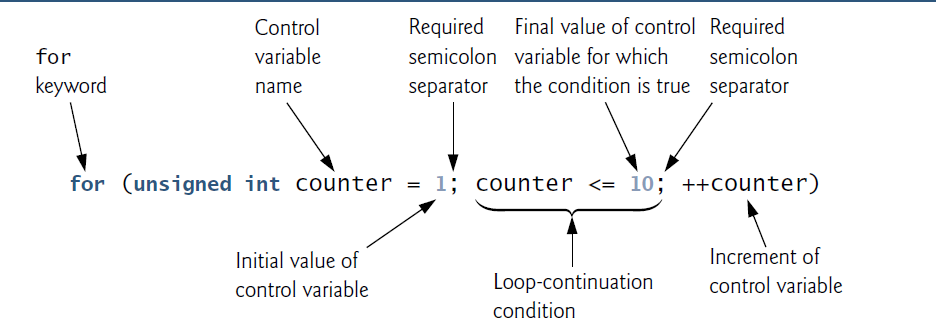
\includegraphics[width=7cm]{CicloFor}
	\end{figure}
	Ejemplo: Hacer un ciclo for que haga lo siguiente:
	\begin{itemize}
		\item Que varie la señal de control en pasos de 7, y que vaya desde 7 hasta 77
		\item Que vaya de 20 a 2, en decremento de a 2.
		\item Varie la señal de control sobre la siguiente secuencia 44,33,22,11,0.
	\end{itemize}
\end{frame}

%%%%%%%%%%%%%%%%% FRAME %%%%%%%%%%%%%%%%%%%%%%%%%%
\begin{frame}
	\frametitle{Ciclos for - Ejemplo}
	Haga un programa que calcule el interes compuesto dado un valor de inversión. El interes compuesto esta dado por $a=p(1+r)^n$, donde $p$ es el valor original invertido, $r$ es la tasa de interes anual, $n$ el número de años, $a$ es el deposito al final del año $n$.
\end{frame}

%%%%%%%%%%%%%%%%% FRAME %%%%%%%%%%%%%%%%%%%%%%%%%%
\begin{frame}[fragile]
	\frametitle{Solución - ejemplo}
		
	\begin{lstlisting}[style=CStyle]
		#include <stdio.h>
		#include <math.h>
		
		int main(void)
		{
			double principal = 1000.0; // starting principal
			double rate = .05; // annual interest rate
			
			// output table column heads
			printf("% 4s% 21s\n", "Year", "Amount on deposit");
			
			// calculate amount on deposit for each of ten years
			for (unsigned int year = 1; year <= 10; ++year) {
			
			// calculate new amount for specified year
			double amount = principal * pow(1.0 + rate, year);
			
			// output one table row
			printf("% 4u% 21.2f\n", year, amount);
			}
		}
	\end{lstlisting}
	
\end{frame}

%%%%%%%%%%%%%%%%% FRAME %%%%%%%%%%%%%%%%%%%%%%%%%%
\begin{frame}[fragile]
	\frametitle{Observaciones ciclos for}
	\begin{itemize}
		\item La inicialización, la condición de iteración y el incremento pueden contener operaciones aritméticas. Por ejemplo:  
		\begin{lstlisting}[style=CStyle]
			for (j = x; j <= 4 * x * y; j += y / x)
		\end{lstlisting}
		\item El incremento puede ser negativo. Cuenta de forma descendente.
		\item Si la condición del \textit{loop} es falsa al inicio, el for no se ejecuta ninguna vez.
		\item El usual no usar la variable de control dentro del loop.
		\item El ciclo \textit{for} es como una secuencia de flujo. 
		\begin{figure}
			\centering
			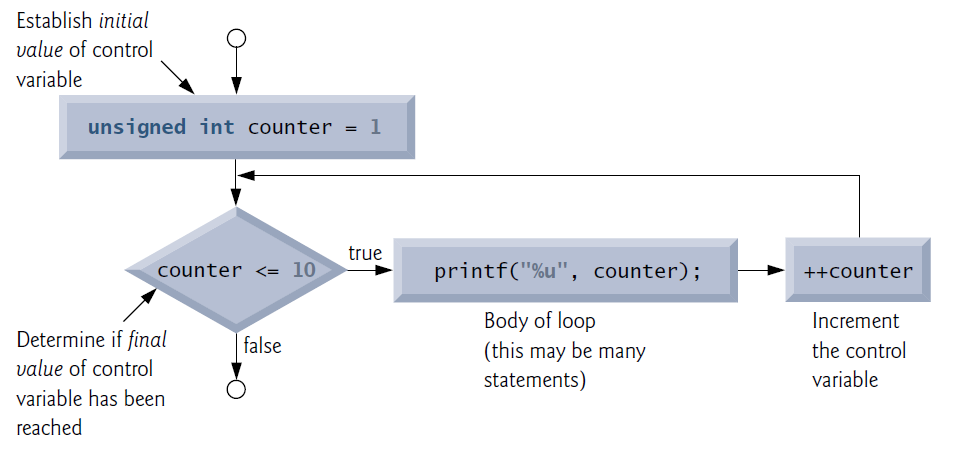
\includegraphics[scale=0.5]{FlowchartFor}
		\end{figure}
	\end{itemize}
\end{frame}
%%%%%%%%%%%%%%%%% FRAME %%%%%%%%%%%%%%%%%%%%%%%%%%
\begin{frame}
	\frametitle{Ciclos do... while}
	Es muy similar al ciclo while, con la variante que se asegura ejecutar al menos una vez el ciclo. 
	\begin{figure}
		\centering
	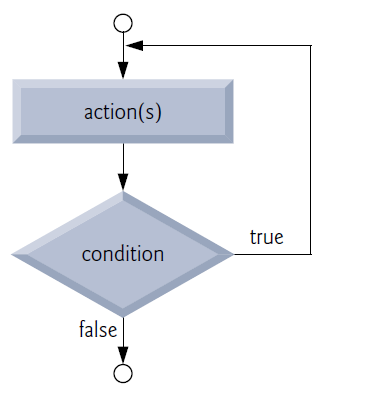
\includegraphics[width=5cm]{DoWhile}
	\end{figure}
	En el diagrama se observa que la acción dentro del ciclo se ejecuta y luego se realiza la pregunta de la condición. 
\end{frame}

%%%%%%%%%%%%%%%%% FRAME %%%%%%%%%%%%%%%%%%%%%%%%%%
\begin{frame}[fragile]
	\frametitle{Ejemplo do... while}
	\begin{lstlisting}[style=CStyle]
		#include <stdio.h>
		
		int main(void)
		{
			unsigned int counter = 1;
			
			do{
				printf("% u ", counter);
			}while(++counter<=10);
		}
	\end{lstlisting}
	En el ejemplo se tiene un ciclo controlado por contador
	
	\textbf{Nota}: Las palabras \textbf{break} y \textbf{continue} son utilizadas en C para terminar un ciclo de forma abrupta o saltarse una iteracion del mismo. 
\end{frame}

%%%%%%%%%%%%%%%%% FRAME %%%%%%%%%%%%%%%%%%%%%%%%%%
\begin{frame}[fragile]
	\frametitle{Ejemplo break}
	\begin{lstlisting}[style=CStyle]
		#include <stdio.h>
		
		int main(void)
		{
			unsigned int x; // declared here so it can be used after loop
			
			// loop 10 times
			for (x = 1; x <= 10; ++x) {
				// if x is 5, terminate loop
				if (x == 5) {
					break;// break loop only if x is 5
				}
				printf("% u ", x);
			}
			printf("\nBroke out of loop at x == % u\n", x);
		}
	\end{lstlisting}
	A pesar de que el \textit{for} esta estructurado para ejecutarse 10 veces, no lo hará debido a la instrucción \textit{break} con la condición que se impone.
\end{frame}

%%%%%%%%%%%%%%%%% FRAME %%%%%%%%%%%%%%%%%%%%%%%%%%
\begin{frame}[fragile]
	\frametitle{Ejemplo continue}
	\begin{lstlisting}[style=CStyle]
		// Using the continue statement in a for statement.
		#include <stdio.h>
		
		int main(void)
		{
			// loop 10 times
			for (unsigned int x = 1; x <= 10; ++x) {
				// if x is 5, continue with next iteration of loop
				if (x == 5) {
					continue;// skip remaining code in loop body
				}
				printf("% u ", x);
			}
			puts("\nUsed continue to skip printing the value 5");
		}
	\end{lstlisting}
\end{frame}


%%%%%%%%%%%%%%%%% FRAME %%%%%%%%%%%%%%%%%%%%%%%%%%
\begin{frame}[fragile]
	\frametitle{Operadores Lógicos}
	Operador lógico AND
	\begin{lstlisting}[style=CStyle]
		if (gender == 1 && age >= 65) {
			++seniorFemales;
		}
	\end{lstlisting}

	Operador lógico OR
	\begin{lstlisting}[style=CStyle]
		if (semesterAverage >= 90 || finalExam >= 90) {
			puts("Student grade is A");
		}
	\end{lstlisting}

	Operador lógico negacion
	\begin{lstlisting}[style=CStyle]
		if (!(grade == sentinelValue)) {
			printf("The next grade is %f\n", grade);
		}
	\end{lstlisting}
\end{frame}
%%%%%%%%%%%%%%%%% FRAME %%%%%%%%%%%%%%%%%%%%%%%%%%
\begin{frame}
	\frametitle{Detección de errores}
	\begin{figure}
		\centering
		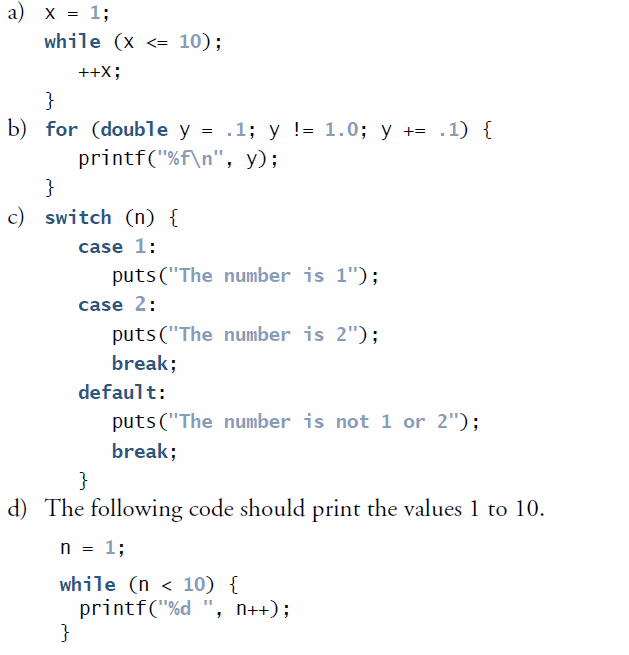
\includegraphics[scale=0.7]{DeteccionErrores}
	\end{figure}
\end{frame}

%%%%%%%%%%%%%%%%% FRAME %%%%%%%%%%%%%%%%%%%%%%%%%%
\frame{
	\frametitle{Ejercicios}
	\begin{itemize}
		\item Suma y promedio de enteros: escriba un programa que sume la secuencia de número enteros y calcule el promedio. Asuma que el primer entero indicará cuantos enteros va a leer. Tu programa debe leer un numero al tiempo. 
		\item Haga un programa que convierta de Farenheit a Celsius.
		\item Haga un programa que calcule el factorial de un número.
		\item Haga un programa que obtenga todos los números primos del 1 al 100.
		\item Escriba un programa que imprima la suma, la suma del cuadrado y la suma del cubo de todos los números naturales del 1 hasta el numero ingresado por el usuario.
	\end{itemize}
}
%%%%%%%%%%%%%%%%% FRAME %%%%%%%%%%%%%%%%%%%%%%%%%%
\frame{
\begin{center}
	\LARGE \textcolor{blue}{PROGRAMACIÓN EN C}
\end{center}

\begin{center}
	\LARGE \textcolor{blue}{GRACIAS}
\end{center}
}

%%%%%%%%%%%%%%%%%%%%%%%%%%%%%%%%%%%%%%%%%%%%%%%%%%%%%%%%%%%%%%%%%%%%%%%%%%%%%%%%%%%%%%%%%%%%%%%%%%%%%%%%%%%%%



\end{document}

